
\chapter{RESULTADOS}

Durante o desenvolvimento deste projeto, foi possível observar como a tecnologia pode contribuir para a organização e o gerenciamento de um escritório de advocacia. A partir das necessidades identificadas, foi desenvolvida a plataforma JurisFlow, com funcionalidades voltadas ao gerenciamento das atividades e das informações utilizadas no dia a dia do escritório.

A plataforma reúne recursos para o cadastro de clientes, organização de pastas e casos, acompanhamento de processos, gerenciamento de diligências e prazos, além do controle de usuários. Dessa forma, o projeto busca facilitar o acesso às informações e contribuir para uma gestão mais organizada das demandas jurídicas.

\section{APRESENTAÇÃO DA PLATAFORMA JURISFLOW}

Nesta seção são apresentadas algumas das principais telas da plataforma, demonstrando como as funcionalidades foram organizadas e disponibilizadas aos usuários.

\subsection{TELAS PRINCIPAIS}

A tela de login é o primeiro acesso à plataforma. Por meio dela, os usuários podem informar suas credenciais para entrar no sistema, de acordo com seu perfil de acesso.

\begin{figure}[H]
    \caption{Tela de login do JurisFlow}
    \centering
    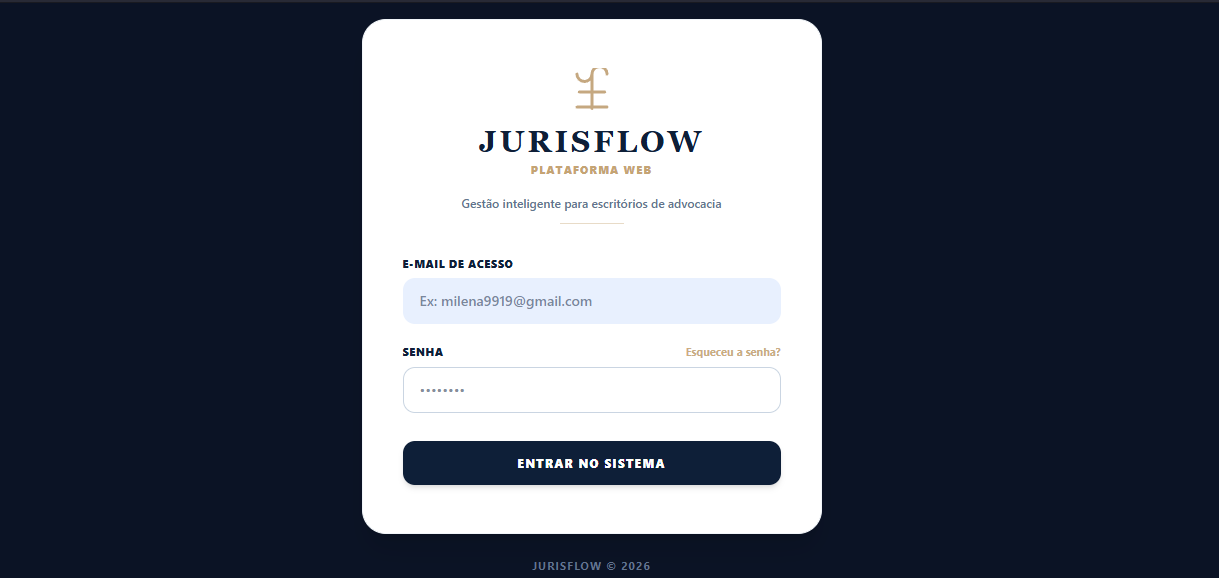
\includegraphics[width=0.9\textwidth]{04-figuras/tela login.png}
    \label{fig:tela-login}
    \fonte{Elaborado pelos autores (2026).}
\end{figure}

Após a autenticação, o usuário é direcionado para a área principal do sistema, onde pode acessar as funcionalidades disponíveis de acordo com suas permissões.

\subsection{FUNCIONALIDADES IMPLEMENTADAS}

O JurisFlow reúne seis funcionalidades principais, desenvolvidas para atender às necessidades identificadas durante o planejamento do projeto.

\subsubsection{Gerenciamento de usuários e controle de acesso}

O sistema possui um módulo de gerenciamento de usuários, no qual o administrador-chefe pode realizar o cadastro, a edição e a exclusão de usuários, além de definir suas permissões. Foram estabelecidos diferentes perfis de acesso, considerando as responsabilidades de cada usuário dentro do escritório. O perfil de advogado e assistente jurídico possuem acesso às mesmas funcionalidades, enquanto o administrador-chefe também é responsável pelo gerenciamento dos usuários.

\begin{figure}[H]
    \caption{Tela de cadastro de membro da equipe}
    \centering
    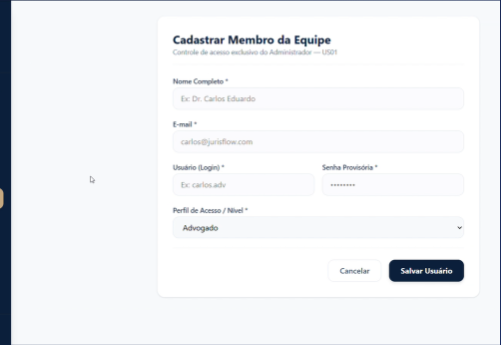
\includegraphics[width=0.9\textwidth]{04-figuras/cadastro membro da equipe.png}
    \label{fig:cadastro-membro}
    \fonte{Elaborado pelos autores (2026).}
\end{figure}

\subsubsection{Cadastro e gerenciamento de clientes}

A plataforma permite cadastrar clientes e armazenar suas principais informações. Também é possível consultar, editar e excluir os registros. Essa funcionalidade facilita a organização dos dados e permite que os usuários encontrem as informações dos clientes com mais facilidade.

\begin{figure}[H]
    \caption{Tela de cadastro de cliente}
    \centering
    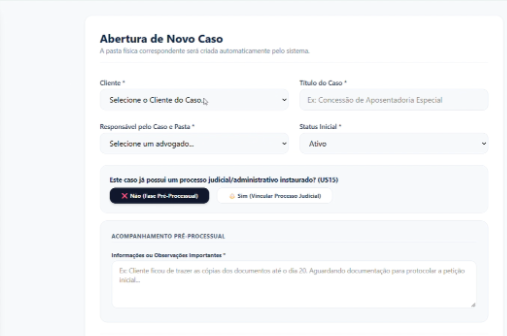
\includegraphics[width=0.9\textwidth]{04-figuras/cadastro de cliente.png}
    \label{fig:cadastro-cliente}
    \fonte{Elaborado pelos autores (2026).}
\end{figure}

\subsubsection{Gerenciamento de casos}

O sistema permite criar casos para organizar as demandas dos clientes e registrar os processos relacionados a cada um. Os casos podem ser classificados como pré-processuais ou processuais, facilitando a identificação de cada demanda e permitindo acompanhar sua situação dentro do escritório.

\begin{figure}[H]
    \caption{Tela de gestão de casos}
    \centering
    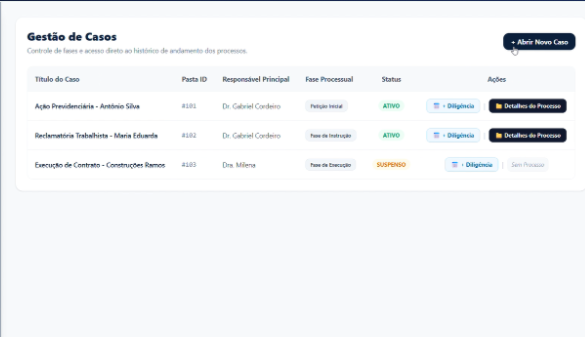
\includegraphics[width=0.9\textwidth]{04-figuras/gestao de casos.png}
    \label{fig:gestao-casos}
    \fonte{Elaborado pelos autores (2026).}
\end{figure}


\subsubsection{Acompanhamento de processos}

A plataforma permite registrar processos judiciais e relacioná-los aos casos já cadastrados. Dessa forma, as informações ficam organizadas em um mesmo ambiente, facilitando a consulta e o acompanhamento pelos profissionais do escritório.

\begin{figure}[H]
    \caption{Tela de detalhes do processo}
    \centering
    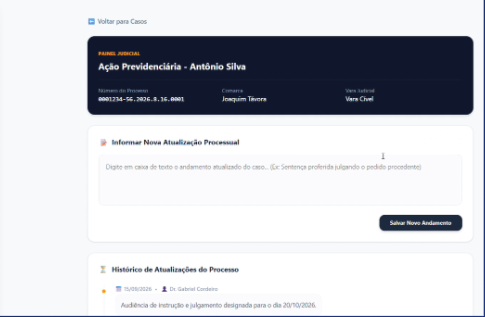
\includegraphics[width=0.9\textwidth]{04-figuras/detalhes de processo.png}
    \label{fig:detalhes-processo}
    \fonte{Elaborado pelos autores (2026).}
\end{figure}

\subsubsection{Gerenciamento de diligências e prazos}

O gerenciamento de diligências permite registrar atividades que precisam ser realizadas em cada caso ou processo. Também é possível organizar os prazos relacionados a essas atividades, ajudando os profissionais a acompanhar suas responsabilidades e evitar que informações importantes sejam esquecidas.

\begin{figure}[H]
    \caption{Tela de cadastro de diligência}
    \centering
    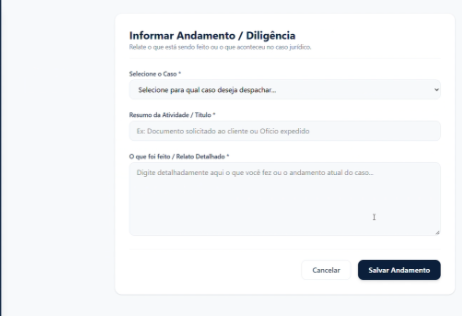
\includegraphics[width=0.9\textwidth]{04-figuras/cadastro de diligencia.png}
    \label{fig:cadastro-diligencia}
    \fonte{Elaborado pelos autores (2026).}
\end{figure}

\subsubsection{Dashboard e indicadores gerenciais}

O dashboard apresenta uma visão geral das informações cadastradas no sistema, por meio de indicadores relacionados aos clientes, casos e processos. Com isso, os usuários podem consultar os dados de forma mais rápida e acompanhar as demandas do escritório em um único lugar.

\begin{figure}[H]
    \caption{Dashboard}
    \centering
    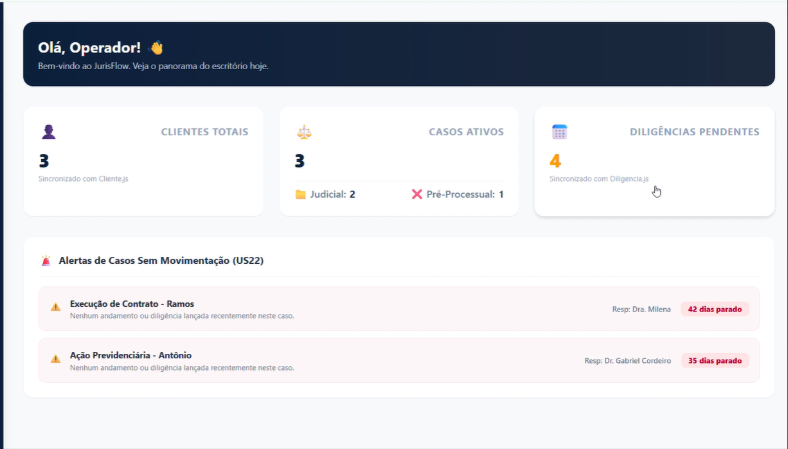
\includegraphics[width=0.9\textwidth]{04-figuras/dashboard chefe admin.png}
    \label{fig:dashboard}
    \fonte{Elaborado pelos autores (2026).}
\end{figure}

\subsection{SEGURANÇA}

Como o JurisFlow trabalha com informações de clientes e processos jurídicos, a segurança foi considerada durante o desenvolvimento da plataforma. Foram utilizados recursos para controlar o acesso dos usuários e proteger as informações armazenadas no sistema.

\subsubsection{Controle de permissões}

Para organizar o acesso ao sistema, foram criados diferentes perfis de usuários, cada um com suas próprias permissões.

Para controlar esse acesso, foi desenvolvido o componente PermissaoGuard, que verifica quais perfis podem acessar cada página do sistema.

Também foi implementado um middleware no backend, responsável por verificar se o usuário tem permissão para realizar determinadas ações. Assim, o controle não acontece apenas nas páginas que o usuário consegue visualizar, mas também nas requisições feitas ao servidor. Quando o usuário não possui a permissão necessária, o acesso à ação deve ser bloqueado.

As Figuras \ref{fig:controle-acesso} e \ref{fig:middleware-permissoes} apresentam os códigos utilizados para realizar esse controle no frontend e no backend.

\begin{figure}[H]
    \caption{Código do componente de controle de permissões}
    \centering
    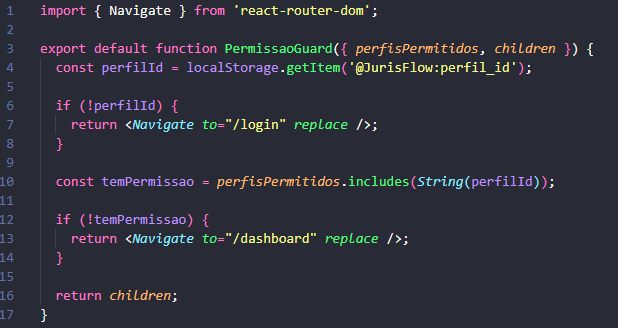
\includegraphics[width=0.9\textwidth]{04-figuras/permissionguard.png}
    \label{fig:controle-acesso}
    \fonte{Elaborado pelos autores (2026).}
\end{figure}

\begin{figure}[H]
    \caption{Código do middleware de controle de permissões}
    \centering
    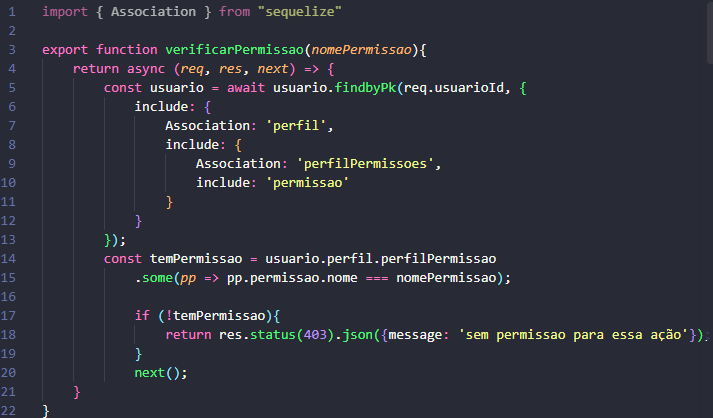
\includegraphics[width=0.9\textwidth]{04-figuras/midllewares permisao.png}
    \label{fig:middleware-permissoes}
    \fonte{Elaborado pelos autores (2026).}
\end{figure}

\subsubsection{Validação de credenciais}

No processo de login, o sistema verifica as informações inseridas pelo usuário para confirmar sua identidade. O acesso é realizado utilizando o login ou e-mail cadastrado e a senha correspondente. Também existe uma verificação para impedir que usuários inativos acessem a plataforma. Após a validação, o sistema gera um token JWT, utilizado para identificar o usuário durante o acesso às demais funcionalidades.

\begin{figure}[H]
    \caption{Implementação da validação de credenciais}
    \centering
    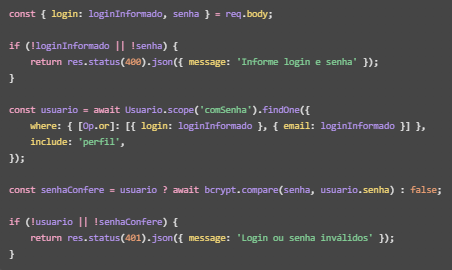
\includegraphics[width=0.9\textwidth]{04-figuras/Validação das credenciais.png}
    \label{fig:validacao-login}
    \fonte{Elaborado pelos autores (2026).}
\end{figure}

\begin{figure}[H]
    \caption{Implementação da geração do token JWT}
    \centering
    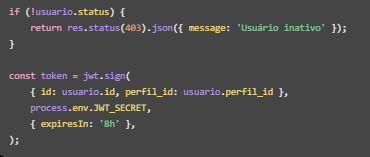
\includegraphics[width=0.9\textwidth]{04-figuras/geração de token JWT.png}
    \label{fig:geracao-token}
    \fonte{Elaborado pelos autores (2026).}
\end{figure}

\subsubsection{Proteção das informações}

Para proteger as senhas dos usuários, foi utilizada a biblioteca bcrypt, que transforma as senhas em hashes antes de armazená-las no banco de dados. Dessa forma, as senhas não ficam salvas em seu formato original. Também foi utilizado o JWT para auxiliar na identificação dos usuários e no controle de acesso às funcionalidades protegidas do sistema.

\begin{figure}[H]
    \caption{Implementação da proteção de senhas}
    \centering
    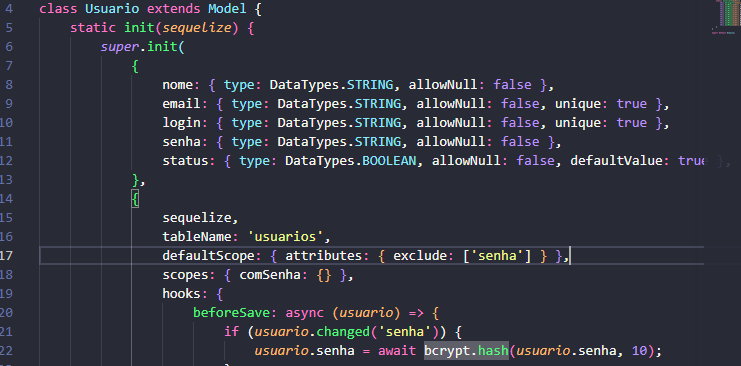
\includegraphics[width=0.9\textwidth]{04-figuras/hash.png}
    \label{fig:protecao-senhas}
    \fonte{Elaborado pelos autores (2026).}
\end{figure}

\section{DISCUSSÃO DOS RESULTADOS}
Apesar dos resultados obtidos, é importante reconhecer algumas limitações da plataforma desenvolvida. O JurisFlow não possui integração com os sistemas dos tribunais, de modo que o registro e a atualização das informações processuais dependem do preenchimento manual pelos usuários. Além disso, a plataforma foi desenvolvida para uso em navegadores web, não havendo, até o momento, uma versão para dispositivos móveis. Outra limitação refere-se à ausência de testes formais com usuários, uma vez que a validação das funcionalidades ocorreu principalmente durante o desenvolvimento, e não por meio de uma avaliação estruturada com profissionais que utilizariam o sistema no dia a dia.